% --
% adversarial

\section{Adversarial Pre-Training}\label{sec:nn_adv}
In adversarial neural network training, two separate neural networks are competing against each other in an adversary task.
This competition of the two networks motivates them to improve their performance and beat the other network.
The application of GANs, as already explained in \rsec{prev_nn_adv} and \rsec{nn_theory_gan}, is an interesting subject in research and the questions whether the obtained weights from the training of the Generator (G) and Discriminator (D) network can contribute to better the performances in equivalent models, arises.
In the following, the training algorithms are explained in more detail, such as the loss functions used for G and D.
The transfer of weights can be done for training instances on small subsets of labels or the whole network by regarding all labels at once in a single training instance.
The transferring technique of training instances on small subsets of labels is denoted as \emph{adversarial label train} and the transfer of weights from a whole network with all labels is named as \emph{adversarial dual train}.
Further those training techniques are explained, except of the adversarial dual train, because it is straight forward once the adversarial label train is understood.


% --
% training GANs

\subsection{Training Generative Adversarial Neural Networks}
The interesting part in training GANs is how the Generator (G) and Discriminator (D) models are updated in each training step and which loss functions were used.
In \req{nn_theory_gan} the game is notated as min-max game, from which the loss of D $l_D$ can be described for one specific training example $i$ of a batch as:
\begin{equation}
  l_D(x_i, z_i, G) = l(D(x_i), y_r) + l(D(G(z_i)), y_f)
\end{equation}
where $l$ is the binary cross-entropy loss described in \req{nn_theory_binary_cross_entropy}, $D: \mathcal{X} \mapsto [0, 1]$ and $G: \mathcal{Z} \mapsto \mathcal{X}$, $x_i \in \mathcal{X}$ is the data example, $z_i \in \mathcal{Z}$ is a randomly sampled latent variable, $y_r = 1$ is the real label and $y_f = 0$ the fake label for that specific example $i$.
In contrast the loss of the Generators $l_G$ is given by:
\begin{equation}
  l_G(z_i, D) =  l(D(G(z_i)), y_r)
\end{equation}
with $y_r$ as real label to perform maximization of $\log D(G(\bm{z}))$ as described in \rsec{nn_theory_gan}.
An extended approach, so that G produces samples specifically similar to the data distribution and does not drift off into creating unrealistic fakes of noisy samples to fake D, is to incorporate a similarity term with the \emph{cosine similarity} defined by:
\begin{equation}
  s(\bm{x_1}, \bm{x_2}) = \frac{\bm{x_1}^T \bm{x_2}}{\norm{\bm{x_1}}_2 \cdot \norm{\bm{x_2}}_2 + \epsilon} 
\end{equation}
where $s : (\mathcal{X}, \mathcal{X}) \mapsto [0, 1]$ is the cosine similarity function, $\bm{x_1}$ and $\bm{x_2}$ are two vectors for similarity measure and $\epsilon$ is a small number, such that no division by zero is possible.
With the similarity loss incorporated, $l_G$ gets:
\begin{equation}
  l_G(x_i, z_i, D) =  l(D(G(z_i)), y_r) + \lambda \left(1 - \frac{1}{C} \sum_{c=0}^{C} s(\hat{\bm{e}}_c^T x_i , \hat{\bm{e}}_c^T G(z_i)) \right)
\end{equation}
where $\hat{\bm{e}}_c \in \{1, 0\}^C$ is a unit vector representing one cepstral coefficient of the Mel Frequency Cepstral Coefficient (MFCC) data $x_i \in \mathcal{X} = \R^{C \times M}$ with a total number of $C$ MFCC coefficients and $M$ frames.
Further $\lambda$ is a trade-off factor between data similarity and fake loss from D.
For the experiments in \rsec{exp_adv}, $\lambda = 5$ was chosen.

The update of D and G is performed in each training step by backpropagating the obtained losses.
However it is more appealing if D is updated for a certain numbers of training steps with no update of G and then alternating to updates of G without updating D.
This will give either D or G some update steps to improve in their specific adversarial task of either discriminating or generating.
In this thesis the training steps for updating either D or G were selected to 2 epochs.
Note that an epoch consists of several training steps depending on the batch size and amount of data.
This can vary for the experiments, however it does not dramatically influence the overall end results.


% --
% label train

\subsection{Adversarial Label Train}
Adversarial label train, is the transfer of weights from feature maps trained on multiple GAN training instances on subsets of all labels.
For instance if the total amount of labels are \{\enquote{left}, \enquote{right}\} then an own training instance may focus on the label \enquote{left} and another on the label \enquote{right}.
It is important to assign a specific number of feature maps to each label train instance, for example each label train gets 8 feature maps of the first convolutional layers.
The label train scheme is illustrated in \rfig{nn_adv_label_scheme} and applies 6 label train instances, such as used for the experiments in \rsec{exp_adv}.
\begin{figure}[!ht]
  \centering
    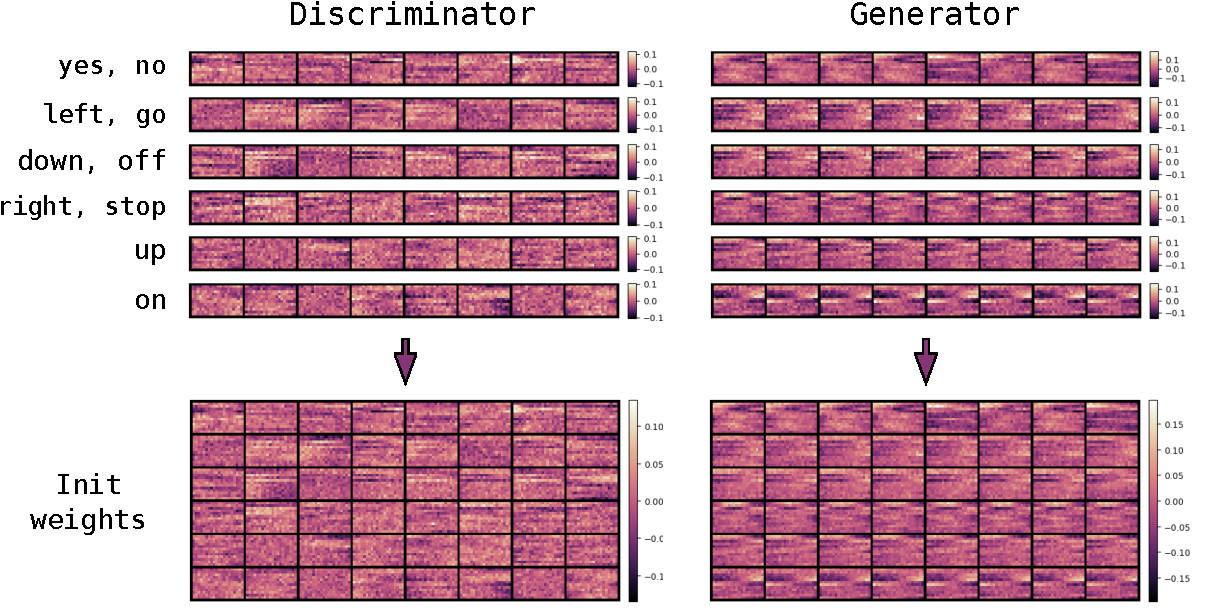
\includegraphics[width=0.7\textwidth]{./4_nn/figs/nn_adv_label_scheme.pdf}
  \caption{Label train scheme of 6 training instances, trained with 100 epochs for each label subset.}
  \label{fig:nn_adv_label_scheme}
\end{figure}
\FloatBarrier
\noindent
An actual GAN training for the labels \enquote{left} and \enquote{go} is shown in \rfig{nn_adv_loss_label}.
Note that the update of either the Discriminator (D) or Generator (G) model is done alternating for 2 training epochs.
\begin{figure}[!ht]
  \centering
  \subfigure[it-100]{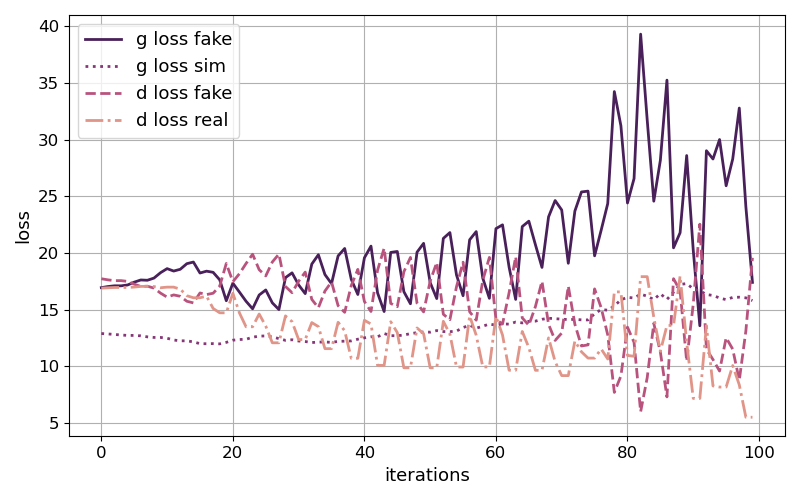
\includegraphics[width=0.45\textwidth]{./4_nn/figs/nn_adv_loss_label_it-100.png}}
  \subfigure[it-1000]{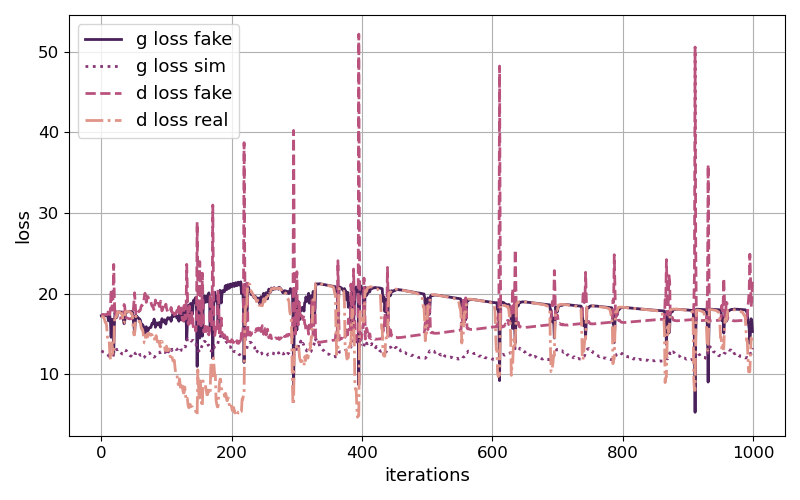
\includegraphics[width=0.45\textwidth]{./4_nn/figs/nn_adv_loss_label_it-1000.png}}
  \caption{Adversarial training loss of the labels \enquote{left} and \enquote{go} with 8 feature maps.}
  \label{fig:nn_adv_loss_label}
\end{figure}
\FloatBarrier
\noindent
The creation of fake images from G is shown in \rfig{nn_adv_fakes_label} of the same training instances.
\begin{figure}[!ht]
  \centering
  \subfigure[it-100]{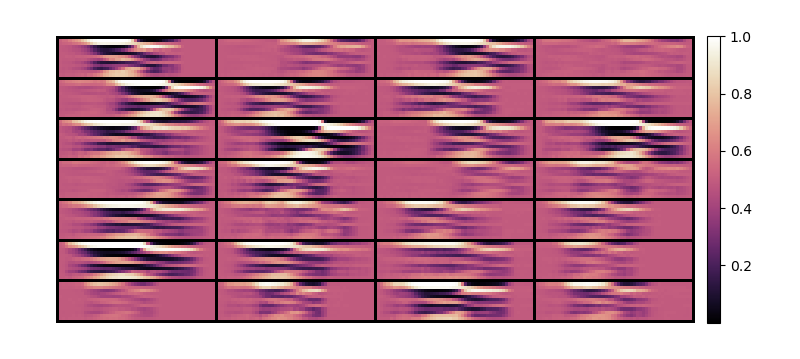
\includegraphics[width=0.45\textwidth]{./4_nn/figs/nn_adv_fakes_label_it-100.png}}
  \subfigure[it-1000]{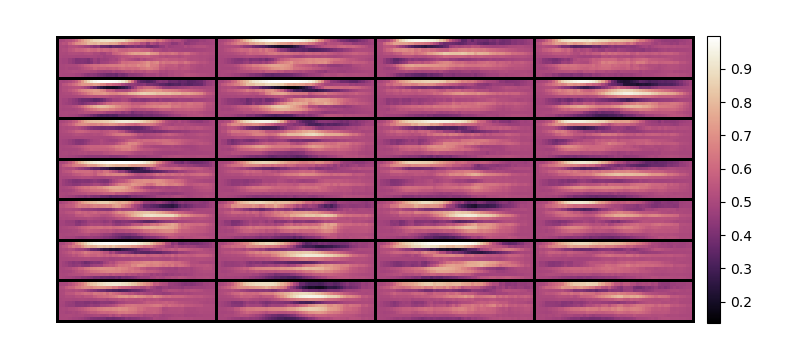
\includegraphics[width=0.45\textwidth]{./4_nn/figs/nn_adv_fakes_label_it-1000.png}}
  \caption{Generation of fake images of the labels \enquote{left} and \enquote{go} with 8 feature maps for the GAN training.}
  \label{fig:nn_adv_fakes_label}
\end{figure}
\FloatBarrier
\noindent

As showcase example, some concatenated adversarial label train weights used for weight transfer, are shown for D and G with different amounts of training epochs in \rfig{nn_adv_label_weights_d} and \rfig{nn_adv_label_weights_g}.
\begin{figure}[!ht]
  \centering
  \subfigure[d-100]{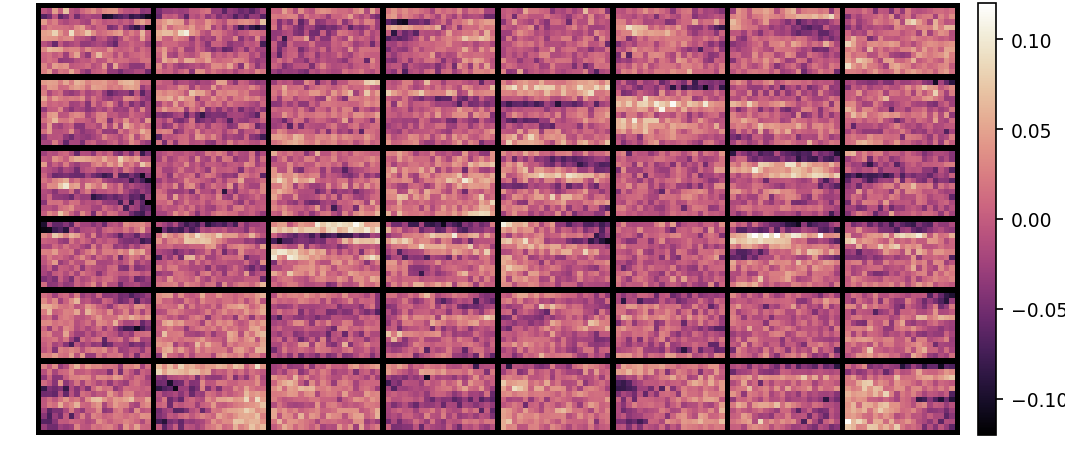
\includegraphics[width=0.45\textwidth]{./4_nn/figs/nn_adv_label_weights_d-100.png}}
  \subfigure[d-1000]{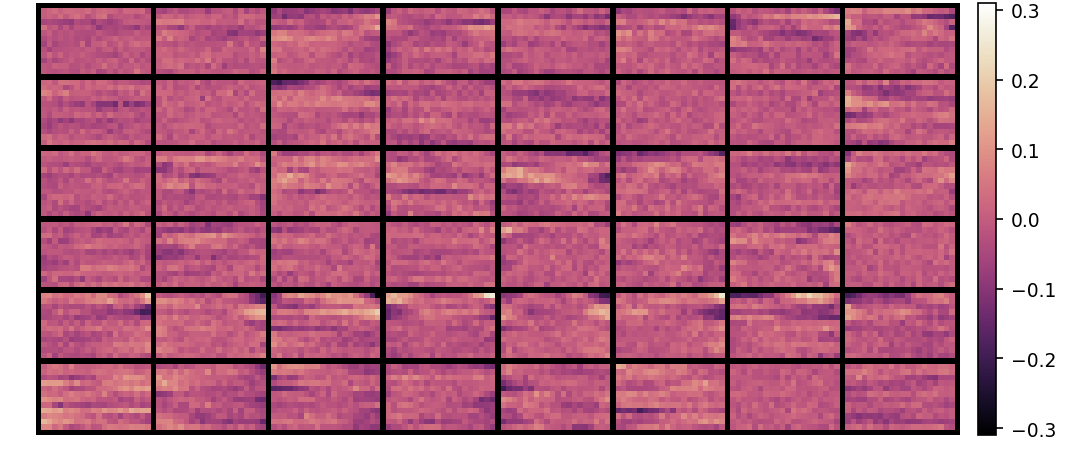
\includegraphics[width=0.45\textwidth]{./4_nn/figs/nn_adv_label_weights_d-1000.png}}
  \caption{Concatenated label weights of the first convolutional layer from the Discriminator model with different amounts of epochs.}
  \label{fig:nn_adv_label_weights_d}
\end{figure}
\FloatBarrier
\noindent
\begin{figure}[!ht]
  \centering
  \subfigure[g-100]{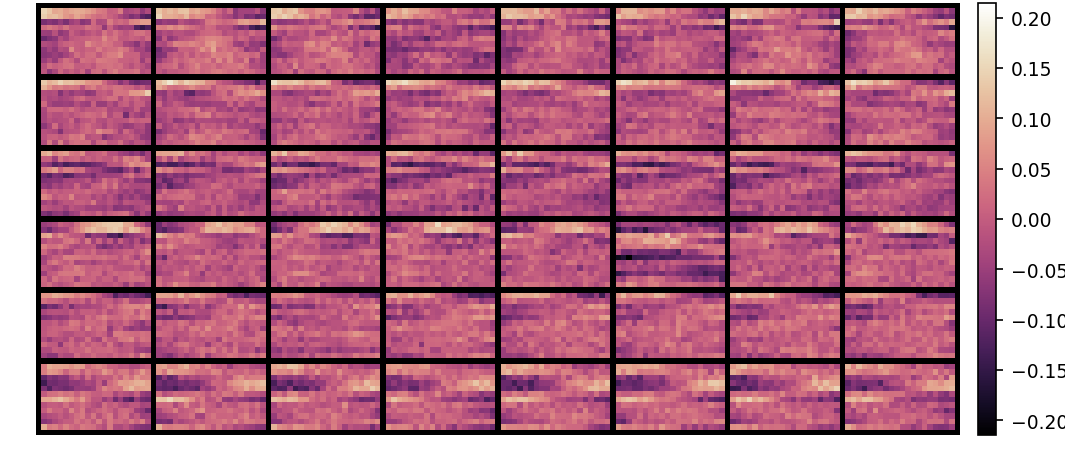
\includegraphics[width=0.45\textwidth]{./4_nn/figs/nn_adv_label_weights_g-100.png}}
  \subfigure[g-1000]{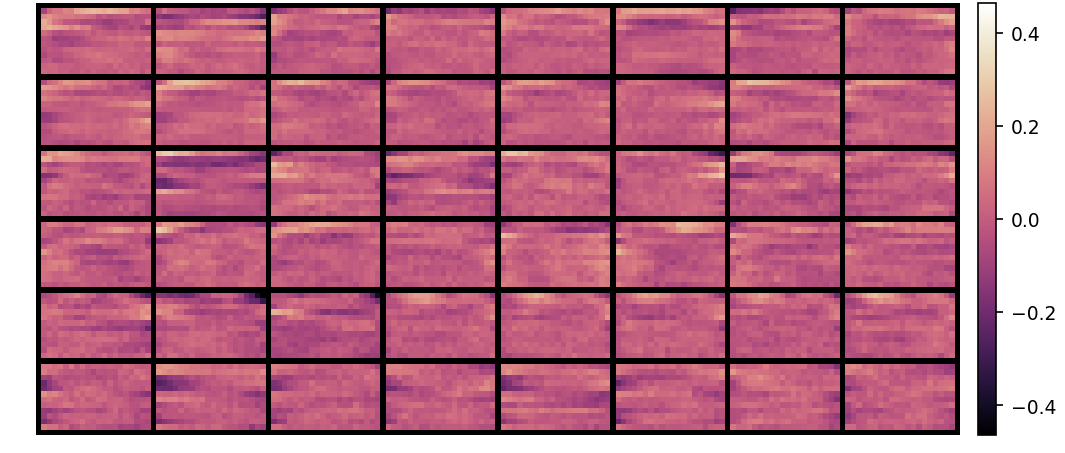
\includegraphics[width=0.45\textwidth]{./4_nn/figs/nn_adv_label_weights_g-1000.png}}
  \caption{Concatenated label weights of the first convolutional layer from the Generator model with different amounts of epochs.}
  \label{fig:nn_adv_label_weights_g}
\end{figure}
\FloatBarrier
\noindent
The amounts of epochs are important, because they determine how much the models are learning in their adversarial task.
With 100 epochs the Generator creates similar feature maps for each label train instance, because it does not need to be that accurate in creating different looking fakes, however the Discriminator gets better as well and the need of generating different looking fakes are necessary to match up.
With 1000 epochs the Generator produces already different fakes as already shown in \rfig{nn_adv_fakes_label} however it is not recommended to train for too long.
Note that a second convolutional layer for the \texttt{adv-d-jim} and \texttt{adv-g-jim} exist as well, the corresponding weights are shown only for the 100 epoch examples in \rfig{nn_adv_label_weights_conv1}.
\begin{figure}[!ht]
  \centering
  \subfigure[d-100]{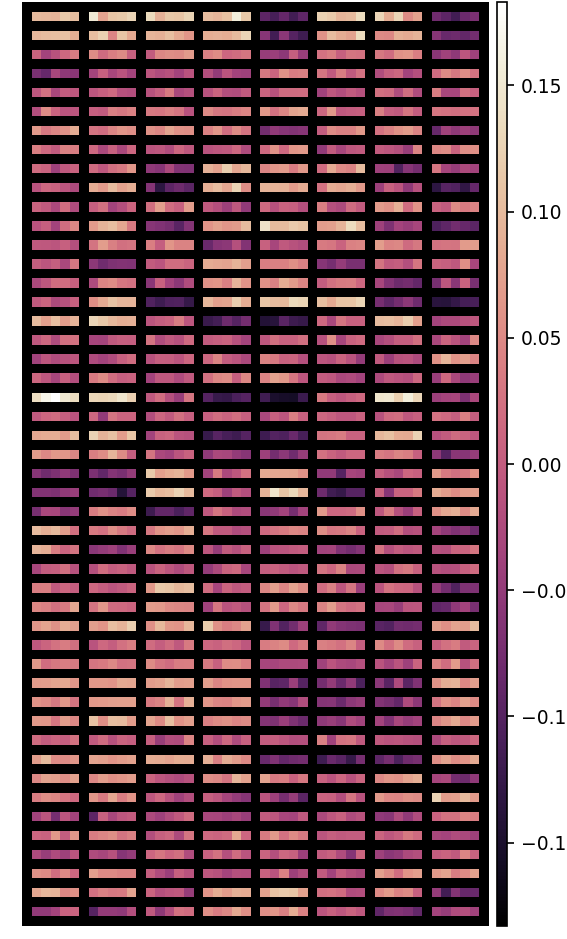
\includegraphics[width=0.25\textwidth]{./4_nn/figs/nn_adv_label_weights_conv1_d-100.png}}
  \qquad \qquad
  \subfigure[g-100]{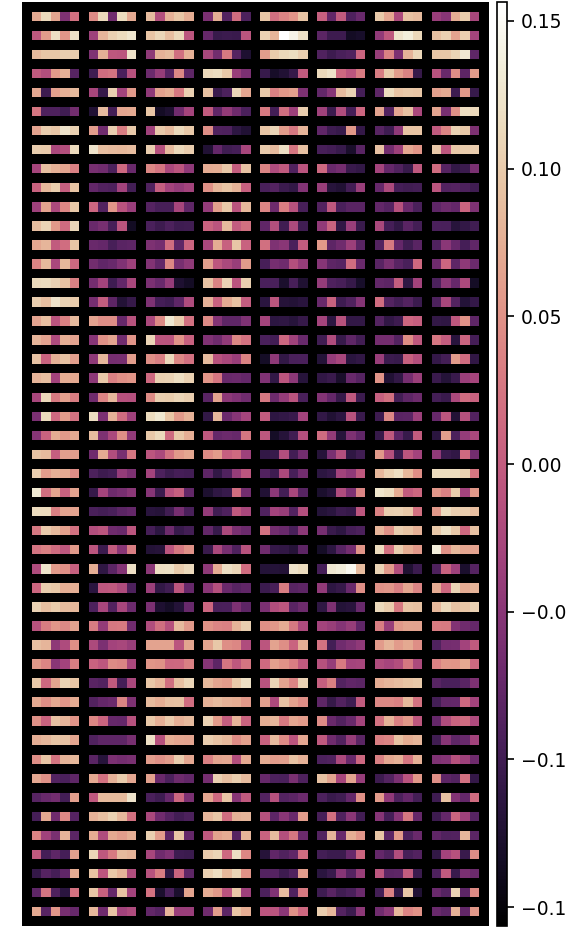
\includegraphics[width=0.25\textwidth]{./4_nn/figs/nn_adv_label_weights_conv1_g-100.png}}
  \caption{Concatenated label weights of the second convolutional layer from the Discriminator and Generator model with trained with 100 epochs.}
  \label{fig:nn_adv_label_weights_conv1}
\end{figure}
\FloatBarrier
\noindent
From the second convolutional layer each row corresponds to a single feature map and therefore 8 rows to one adversarial label training instance.